\section{Particle Orbits}
\begin{frame}{Particle Orbits}
    \begin{itemize}
        \item Particles with high velocity can go around the torus.
        \item Particles with low velocity will be trapped due to mirror effect.
    \end{itemize}
    \begin{figure}
        \centering
        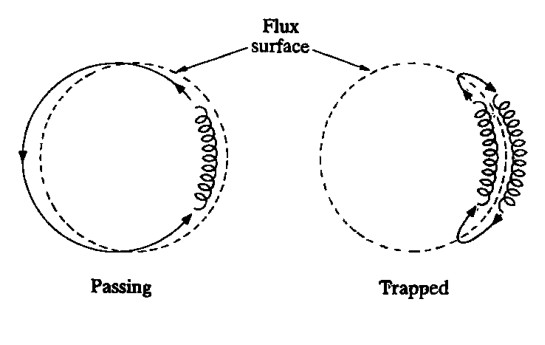
\includegraphics[width=0.7\textwidth]{figures/drift-surface.png}
        \caption{Diagram illustrating drift surfaces for the orbit of a passing particle and the (banana) orbit of a trapped particle. The major axis of the torus is on the left.}
        \label{fig:drift-surfaces}
    \end{figure}
\end{frame}

\begin{frame}{Particle Trapping}
    \begin{itemize}
        \item The vacuume toroidal magnetic field is propotional to $1/R$, the field is smaller on the outer side of the torus.
        \item Particles with a small $v_\parallel$ undergo a magnetic mirror reflection as they move into the region of higher field.
    \end{itemize}
    \begin{figure}
        \centering
        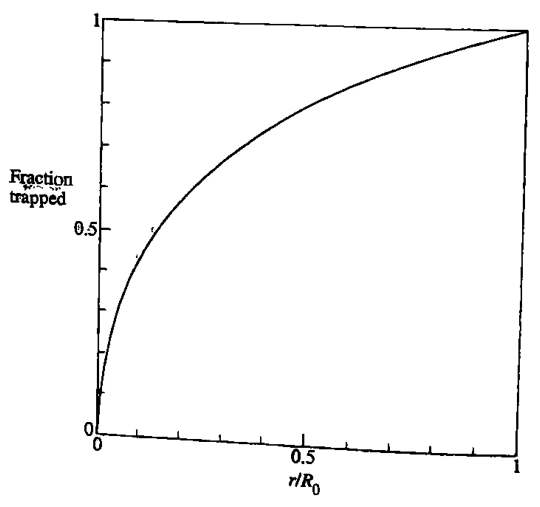
\includegraphics[width=0.4\textwidth]{figures/fraction-trapped.png}
        \caption{Graph of the fraction of the particles which are trapped as a function of the inverse aspect-ratio of the magnetic surface, $r/R_0$.}
        \label{fig:fraction-trapped}
    \end{figure}
\end{frame}

\begin{frame} {Particle Orbits - Banana Orbit}
    \begin{itemize}
        \item For deuterons, $r^{3/2} \gg q\rho R^{1/2} \sim 10^0$\unit{\cm}, so their orbits usually have banana shape.
    \end{itemize}
    \begin{figure}
        \centering
        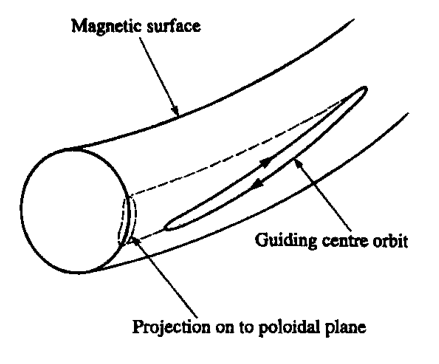
\includegraphics[width=0.7\textwidth]{figures/banana-orbit.png}
        \caption{Showing the banana orbit of a trapped particle with its projection onto a poloidal plane.}
        \label{fig:banana-orbit}
    \end{figure}
\end{frame}

\begin{frame} {Trapped Particle Orbit - Potato Orbits}
    \begin{itemize}
        \item $\alpha$-particles have large Larmor radius and are predominantly produced in the core of plasma, their orbits are called potato orbit.
        \item The potato orbit is given by
              \[ \left(\frac{r}{R_0}\right)^3 = \left(\frac{2\rho q}{R_0}\right)^2\cos\theta \]
              where $q=B/R_0B_\theta'$.
    \end{itemize}
    \begin{figure}
        \centering
        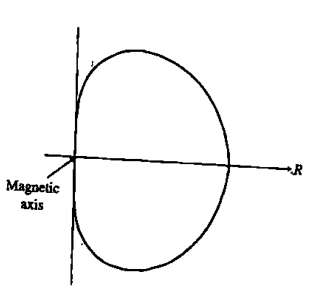
\includegraphics[width=0.3\textwidth]{figures/potato-orbit.png}
        \caption{Potato orbit for particle passing through the magnetic axis.}
        \label{fig:potato-orbit}
    \end{figure}
\end{frame}